\documentclass[10pt]{article}
% TMLR submission format (tmlr.sty / tmlr.bst from github.com/JmlrOrg/tmlr-style-file, Apache-2.0).
% Rev1 preprint: \usepackage[preprint]{tmlr}. Anonymous TMLR: \usepackage{tmlr}.
% If accepted: \usepackage[accepted]{tmlr} and set \month, \year, \openreview below.
\usepackage[preprint]{tmlr}

\usepackage[utf8]{inputenc}
\usepackage[varqu,scaled=0.95]{zi4}   % Inconsolata: a monospace with a real bold
\usepackage{textcomp}                % \textminus: a true minus sign, the width of +, so signed columns align
\usepackage{booktabs}
\usepackage{array}
\usepackage{amsmath}
\usepackage{graphicx}
\usepackage{xcolor}
\usepackage{pgfplots}
\pgfplotsset{compat=1.18}
\usepackage[htt]{hyphenat}
\usepackage{microtype}
\usepackage[font=small, labelfont=bf, skip=6pt]{caption}
\usepackage{enumitem}
\usepackage[title]{appendix}
\usepackage{hyperref}
\usepackage{xurl}   % bibliography URLs may break anywhere

\definecolor{linkblue}{HTML}{1F4E8C}
\hypersetup{colorlinks=true, linkcolor=linkblue, citecolor=linkblue, urlcolor=linkblue,
  pdftitle={Six Pitfalls in Measuring the Cost of Coding Agents},
  pdfauthor={Max Reischl, Alexander Feurer}}

\setlength{\emergencystretch}{3em}
\raggedbottom   % tmlr.sty sets flushbottom, which stretches pages around the unbreakable tables
\setlist{itemsep=2pt, topsep=4pt}
\newcolumntype{L}[1]{>{\raggedright\arraybackslash}p{#1}}
\newcommand*{\mi}{\textminus}   % a minus sign in running text and tables
% a table set where it is discussed, numbered and captioned like a float
\newenvironment{inlinetable}{\par\medskip\noindent\begin{minipage}{\linewidth}\centering\small}{\end{minipage}\par\bigskip}
\newsavebox{\pitbox}
\newenvironment{pitfall}[1]{\par\medskip\noindent\begin{lrbox}{\pitbox}\begin{minipage}{\dimexpr\linewidth-2\fboxsep-2\fboxrule\relax}\small\textbf{#1}\enskip}{\end{minipage}\end{lrbox}\fbox{\usebox{\pitbox}}\par\medskip}

\title{Six Pitfalls in Measuring the Cost of Coding Agents:\\
Evidence from a Cross-provider Study of Code Mode}

\author{\name Max Reischl \email reischl\_max@icloud.com \\
      \addr Independent researcher, Vienna, Austria
      \AND
      \name Alexander Feurer \email feureralexander10@gmail.com \\
      \addr Independent researcher, Vienna, Austria}

\def\month{MM}  % camera-ready only
\def\year{YYYY} % camera-ready only
\def\openreview{\url{https://openreview.net/forum?id=XXXX}} % camera-ready only

\begin{document}

\maketitle

\begin{abstract}
Agent benchmarks now report dollars beside accuracy, but cost is usually estimated from
token counts and a single provider's price list, on one task suite, in one run, in one execution
order. We ran a study of code mode---a harness's programmatic tool-calling mode against its native
tool calling---across six models from five providers, alongside four other open-source harnesses, on
two task suites (8,520 planned cells). The protocol was fixed in advance and amended 23 times
(Appendix~\ref{app:prereg}); a replication criterion and a counterbalanced re-run plan were filed
before those data existed. We metered every request at a gateway that records each provider's usage
and cache accounting, validated to 0.023\% on one 62-run Anthropic development pilot whose raw logs
are not in the checksummed artifact.
On the second suite, code mode (PTC against native) was cheaper for DeepSeek and gpt-6-luna:
\mi{}21.8\% [\mi{}37.46, \mi{}9.38] and \mi{}16.6\% [\mi{}24.35, \mi{}8.55] per task
(both intervals exclude zero and both survive Holm), and \mi{}22.64\% [\mi{}39.77, \mi{}9.19] and
\mi{}18.01\% [\mi{}25.14, \mi{}10.61] on cells both modes solved. A counterbalanced re-run
reproduced the per-task savings (\mi{}16.8\% [\mi{}29.8, \mi{}6.3] and \mi{}19.0\% [\mi{}29.0, \mi{}9.4]).
Neither saving appears on batch 1. We use the study to quantify six
pitfalls. (1) \emph{Token volume is not cost}: pricing tokens without cache accounting reverses the
point-estimate sign of the code-mode effect for three of six models, whose billed intervals include zero; after Holm correction only Haiku survives on batch 1. (2) \emph{Cache configuration is part of the
treatment}: where the cache breakpoint sat decided whether code mode was cached at all, and moving it
made the same matrix 3.4 times cheaper. (3) \emph{Accounting can be missing}: on one provider's
compatibility endpoint 128.1M input tokens arrived without a cache split, and the study's own cost tool
reported more money than was spent. (4) \emph{Execution order carries cost}: one configuration's cost
varied 1.75--3.82-fold with its slot; the order effect was significant in 1 of 9 re-run rows, and a
counterbalanced re-run did not bring the reversed GLM saving back (within the \mi{}8.1\% to +8.0\% native-arm drift).
(5) \emph{Cost without quality misleads}: on one model, code mode looked 54\% dearer per task but was
101\% dearer per solved task, because it also solved fewer tasks (46 against 60 of 62), and the re-run
reproduced the gap (48 against 62). (6) \emph{One suite is not enough}: two interleaved collections of
identical requests differed by \mi{}5.3\%, with an interval half-width of 11.6\% at 31 tasks, and our
own pre-registered replication on a second suite failed for all four providers. On Claude Haiku 4.5, code mode
is dearer and less reliable on batch 1 (the same per-solved direction appears on the second suite, but those intervals include zero). We give a checklist for cost measurement and release the gateway,
logs and analysis code.
\end{abstract}

\section{Introduction}\label{sec:intro}

Cost has become a first-class outcome in agent evaluation. Accuracy-only leaderboards reward
needlessly expensive agents \citep{kapoor2024agents}; cost-of-pass combines price and success
\citep{erol2025costofpass}; leaderboards now log per-task cost across tens of thousands of rollouts
\citep{kapoor2025hal}; and coding-agent papers report dollar cost on SWE-bench
\citep{jimenez2024swebench,xia2024agentless,zhang2024autocoderover} (about \$0.43 per Lite task for AutoCodeRover). Agentic coding consumes orders of magnitude more
tokens than code chat, and runs of the same task vary widely \citep{bai2026agentspend}, so the stakes
are real.

How cost is \emph{measured}, however, has received far less scrutiny than how accuracy is measured.
A typical cost figure multiplies token counts by one provider's list prices, sometimes assuming no
prompt caching \citep{xu2024theagentcompany}, on one task suite, from one run per configuration, with
configurations run in a fixed order. Each of these choices can bias a cost comparison, and none is
usually tested.

We tested them in the course of a study of \emph{code mode}, a design in which an
agent writes a program that calls its tools instead of issuing one tool call per model request
\citep{wang2024codeact}. Vendors report large token savings from code mode
\citep{anthropic2025codeexecutionmcp,anthropic2025advancedtooluse,cloudflare2026codemode}, while
academic work finds the saving depends on workload \citep{patel2026bitterlesson}. We compared the
programmatic tool-calling mode of an open-source harness with its native mode, on six models from five
providers, alongside four other harnesses, on two task suites. A gateway between every harness and
every provider recorded each provider's own usage block, including the cache split, for every
request.

The study's answer about code mode is mixed. On batch 1 no model was significantly cheaper under
code mode; on the second suite DeepSeek and gpt-6-luna showed a saving that a counterbalanced re-run
reproduced (\S\ref{sec:survives}). The filed replication of the batch-1 pattern failed. The more general result
is what it took to reach that answer. At six points a standard measurement practice would have
changed the conclusion or mis-sized it, and we can quantify each one with the study's own data.

\paragraph{Contributions.}
\begin{enumerate}
\item Six pitfalls in measuring agent cost, each quantified on a real study
(\S\ref{sec:accounting}--\S\ref{sec:inference}): three in cost accounting, one in experimental
design, one in the outcome measure, and one in inference.
\item A checklist that addresses each one (\S\ref{sec:checklist}).
\item A gateway-metered, cross-provider measurement of code mode's billed cost, validated against
provider billing, with a pre-registered replication reported although it failed, and a pre-registered
re-run of the central contrast under counterbalanced order (\S\ref{sec:p4}, \S\ref{sec:survives}).
\item The gateway, run records, logs and analysis code, with every reported number re-derivable
(Appendix~\ref{app:artifact}). Unlike the largest public agentic trace set, which records
anonymised providers and cached-token counts from human-driven sessions
\citep{nixon2026freeinference}, our logs come from controlled matrices, name each provider, keep the
cache-write count where the provider reports one, and were checked against the provider's bill where
its balance could be read.
\end{enumerate}

\section{Related work}\label{sec:related}

\paragraph{Cost in agent evaluation.} Beyond the work above, Efficient Agents decomposes framework
design into cost-of-pass \citep{wang2025efficientagents}. The closest work, a preregistered
benchmark, treats prompt wording, inference effort and harness policy as interacting factors and
measures cost per successful task, including runs on DSH \citep{weinberger2026promptwaste}. We share
its outcome measure but study the measurement itself: billed against priced cost, execution order, a
noise floor and replication. An enterprise router study argues that a harness's defaults, caching
among them, set the bill \citep{kwartler2026tokenomics}. Production gateway data report per-agent
cache hit rates across coding agents \citep{jaigu2026codingagenteconomy}, and an independent CLI
benchmark finds that several agents do not cache at all \citep{kalelioglu2026acodecli}. A cheaper
list price does not guarantee a cheaper run \citep{chen2026pricereversal}, and routers exploit price
differences between models \citep{ong2025routellm,chen2024frugalgpt,ding2024hybridllm,yang2026twinrouterbench}.

\paragraph{Validity of agent evaluation.} Harness choice alone can change tokens per solved task
40-fold \citep{vats2026scaffold}, and changing only a harness's context handling, with model and
task fixed, changes solve rates \citep{lewis2026samemodel}; harness gains are comparable to model
gains and harness effects are heterogeneous across models \citep{han2026harness}; harness-induced
variance can exceed model variance \citep{zhang2026stopcomparing}; a controlled pairing study finds
resolve rates moving by up to 44 points and charged tokens per resolved task by more than
20-fold across harnesses for the same model \citep{zhao2026pairingmatters}; a factorial harness-design
study varies planning, action space and context management with cost effects
\citep{fan2026harnessdesign}; and leading SWE-bench entries are statistically inseparable
\citep{liu2026codingagentsconverged}. One study finds rankings stable under scaffold shift
\citep{ndzomga2026efficient}. Nominally deterministic agent runs vary by several points of pass@1
\citep{bjarnason2026randomness}, and run-count guidance exists for accuracy but not for cost
\citep{blackwell2024reproducible,potamitis2025reasonbench}; a survey finds that no prominent agent
benchmark reports a complete standardised cost record \citep{nageshwaran2026survey}. Repeated
configurations vary in per-cell cost with coefficients of variation of 2.4--8.4\%
\citep{hu2026costinefficient}, and A/A designs have been proposed for accuracy
\citep{kaliyev2026noisefloor}. Failed replications of LLM evaluation claims are published
\citep{schaeffer2023emergent,mirzadeh2024gsmsymbolic,xu2026validationevidence}.

\paragraph{Caching and its measurement.} Claw-SWE-Bench v1 reports per-harness billed cost from
provider billing logs together with per-harness cache hit rates \citep{zheng2026clawswebench}, and a
gateway benchmark publishes per-arm hit rates from spend logs \citep{litellm2026autorouter}.
Caching cuts agent cost by 41--80\% across sessions \citep{lumer2026dontbreakthecache}; identical
runs on open-weight models show harness-dependent cache regimes \citep{arino2026identicalruns}; and a
preregistered benchmark reports that hits are probabilistic and that one provider route returned no
cached tokens for days \citep{weinberger2026promptwaste}. An empirical study of 120 prompt-caching
pull requests finds that mis-integrations are common, often silent, and provider-API heterogeneous
\citep{zhang2026silentcostly}. Anthropic documents that its OpenAI-compatible layer does not support
prompt caching \citep{anthropic2025openaisdk}, and issue reports observed the effect in harnesses
\citep{cline2026issue13667,nousresearch2026issue84506}; other routers forward cache markers
\citep{openrouter2026promptcaching}. Code minification can cut state-in-context agent input tokens
substantially on SWE-bench Verified, with a corresponding drop in resolve rate
\citep{hrubec2026minification}. Serving-side prompt reuse is well studied
\citep{gim2024promptcache,yao2025cacheblend,jiang2024longllmlingua}.

\paragraph{Code mode and tool interfaces.} Executable code as an action space was introduced by
CodeAct \citep{wang2024codeact}. A synthetic study finds a token crossover near a fan-out of 26
calls \citep{patel2026bitterlesson}; a five-interface study places programmatic calling between typed
calls and bash \citep{mak2026isbashallyouneed}; restricting coding agents to one code-execution tool
holds pass rates while costs swing 20--40\% \citep{yang2026restrictingexecutecode}. Vendor
demonstrations report order-of-magnitude token savings when the alternative is stuffing large MCP
catalogs into context (150{,}000$\to$2{,}000 tokens, 98.7\%; or $\sim$99.9\% fewer input tokens for a
2{,}500-endpoint API) \citep{anthropic2025codeexecutionmcp,cloudflare2026codemode}; those figures
measure progressive disclosure of huge HTTP APIs, not billed cost of programmatic versus native
calling inside a coding harness with a small tool catalog. The closest published head-to-head, on
six short deterministic workflows and eight models, finds Code Mode cut mean tokens by 37.6\% and
mean cost by 40.7\% versus native MCP, with regressions on weaker and Gemini-family models
\citep{mbat2026codemode}; that average saving is larger than ours, but the capability-dependent sign
matches, and their workloads are not multi-file coding tasks metered at a multi-provider gateway.
E-Bench reports tool-call and turn cuts across eleven models on synthetic product tasks (MCP calls
$-73.8\%$, turns $-33.6\%$), not cache-aware cross-provider billed dollars
\citep{zheng2026ebench}; a vendor CodeAct agent likewise reports fewer input and output tokens on an
in-house benchmark without a published cache-aware bill reconciliation
\citep{strandsagents2026codeagent}. Large-scale tool-use work studies retrieval over many APIs
\citep{qin2023toolllm}, and a Seal-Tools baseline shows retrieval accuracy falling as the tool set
grows \citep{lumer2025toolshed}; interface design affects success
\citep{yang2024sweagent,sweagentteam2025minisweagent}. Concurrent work reprices three harnesses under
two vendors' price lists \citep{liu2026harnessbuy}.

What is new here is not that cost can be measured at a gateway or that caching matters, both of
which are established, but a quantification of how standard measurement choices change a cost
conclusion, on one cross-provider study with a living, amended protocol.

\section{The study}\label{sec:study}

\subsection{Harnesses and arms}

An \emph{arm} is a harness in a fixed configuration; ten arms ran on every model. Six are conditions
of DeepSeek Harness (DSH, version 0.1.7-rc.2), DeepSeek's open-source coding harness. In its
\emph{native} mode the model sees 24 tool schemas and calls one tool per request. In its \emph{PTC}
(programmatic tool calling) mode the tools are presented as a generated TypeScript SDK behind a single
\texttt{run\_code} tool, and the model writes a program that calls them. The archived requests
confirm 24 and 1 schemas. The six DSH arms cross native/PTC with a context policy (shipped, or
optimized with a tool-result pruner) and a terseness instruction. The central contrast is
\texttt{dsh:ptc} against \texttt{dsh:native}. The other four arms are OpenCode 1.18.30, Cline 3.0.65,
OpenHands 1.16.0 and Goose 1.52.0, run with their own defaults. No harness was patched. We did not
develop DSH and are not affiliated with DeepSeek, but we wrote the DSH study conditions and use DSH
daily, an asymmetry against the external harnesses that we cannot remove.

\subsection{Models, providers and cache regimes}

Six models from five providers (Table~\ref{tab:models}) each form one \emph{matrix} of
10 arms $\times$ tasks $\times$ 2 seeds. Four providers contribute one model each, so model and provider
are confounded except within Anthropic. The cache regime differs by provider: DeepSeek and Z.ai cache
automatically; Qwen, served through Alibaba Cloud's Anthropic-compatible endpoint, receives a
gateway-injected breakpoint on the last tool; on gpt-6-luna the requests travel the OpenAI Responses
path, where configured breakpoints are inert; and on Anthropic the gateway injects static breakpoints
plus the top-level cache field (\S\ref{sec:p2}). Reasoning effort was forced to high for DeepSeek and
GLM and left unset for the others.

\begin{inlinetable}
\captionof{table}{Models, price cards (USD per million tokens) and cache regimes.}\label{tab:models}
\setlength{\tabcolsep}{4pt}
\begin{tabular}{@{}llrrrrrl@{}}
\toprule
model & provider & miss & hit & output & out:in & discount & cache regime \\
\midrule
DeepSeek V4.1 Flash & DeepSeek & 0.15 & 0.003 & 0.60 & 4.00 & 50$\times$ & automatic \\
GLM-5.3-Flash & Z.ai & 0.15 & 0.03 & 0.50 & 3.33 & 5$\times$ & automatic \\
Qwen3.8-Flash & Alibaba Cloud & 0.15 & 0.016 & 0.47 & 3.13 & 9.4$\times$ & breakpoint on last tool \\
gpt-6-luna & OpenAI & 0.10 & 0.01 & 0.50 & 5.00 & 10$\times$ & automatic \\
Claude Haiku 4.5 & Anthropic & 1.00 & 0.10 & 5.00 & 5.00 & 10$\times$ & static + top-level \\
Claude Sonnet 5.5 & Anthropic & 2.00 & 0.20 & 10.00 & 5.00 & 10$\times$ & static + top-level \\
\bottomrule
\end{tabular}
\end{inlinetable}

\subsection{Task suites and population}

\emph{Batch 1} has 31 tasks in five strata (single-step, multi-file, repo-wide, long-horizon,
fetch-heavy) plus a smoke task. Each task is a repository with a prompt and a test suite that fails
on the untouched fixture and is deterministic. A run is \emph{solved} if the harness exits 0 and the
suite passes. The suite runs in the agent's workdir, so an agent can weaken the tests it is graded by
(\S\ref{sec:p5}). \emph{Tasks-b} has 40 tasks, ten in each of four strata. It was written after the
batch-1 results were known, as a replication suite, and is graded by a hidden suite that the agent
cannot read or edit.

Batch 1 has 3,720 planned cells (6 models $\times$ 31 tasks $\times$ 10 arms $\times$ 2 seeds).
The Qwen log contains 621 records because one cell (\texttt{multi-file-feature-flags}, \texttt{dsh:native}, seed 2)
was written twice (an infrastructure failure plus its retry); that failed record is one of two
pre-registered exclusions. The other exclusion drops one luna cell. After both exclusions there are
3,719 analysed cells (Qwen 620, luna 619, the other four models 620). Tasks-b has 4,800 planned cells.
Luna lost one cell, and Haiku lost 447 when the Anthropic account reached its monthly limit mid-matrix,
so Haiku's tasks-b row uses the 353 analysed cells from the 18 tasks that ran first (7 of the 360 cells
those tasks would have produced are missing).

\subsection{Measurement}\label{sec:measurement}

Each harness talks to the provider through an HTTP gateway and holds only a synthetic credential that
encodes the run identifier, so every request's usage joins to its run by construction. The gateway
substitutes the real key, enforces the model, logs every rewrite it applies, and records the
provider's usage block. Per run,
\[
\text{cost\_billed} = \text{fresh}\cdot p_{\text{miss}} + \text{created}\cdot p_{\text{write}} +
\text{hit}\cdot p_{\text{hit}} + \text{output}\cdot p_{\text{out}},
\]
re-derived from the archived token counts. \emph{cost\_cold} prices every input token at the miss
rate. Runs execute in a fresh fixture copy, four at a time, with a 20-minute timeout.

\paragraph{Validation against the bill.} On one 62-run Anthropic development pilot we read the account's credit
balance before and after and computed the pilot's cost from its own gateway log: \$35.5718 computed
against a \$35.58 credit delta, a ratio of 1.00023 (0.023\% relative). The pilot's raw logs are not in
the checksummed artifact (Appendix~\ref{app:artifact}). For the main Anthropic matrices the same ledger
bounds the cost from outside (\S\ref{sec:p3}). The re-run's Haiku matrix, on DSH only, agreed with
the balance to the cent (Appendix~\ref{app:rerun}).

\paragraph{Design and analysis.} Within each (task, seed) block the ten arms run in an order fixed by
a seeded shuffle (\S\ref{sec:p4}). Hypotheses were filed before the six-model matrices ran
(Appendix~\ref{app:prereg}), and a replication criterion for tasks-b was filed before any tasks-b data
existed. The unit is the run, and tasks block. Contrasts are paired by task, with a percentile
bootstrap over tasks ($B = 200{,}000$) on the absolute difference, expressed as a percentage of the
native mean. A contrast is \emph{positive} or \emph{negative} if its 95\% interval excludes zero, and
\emph{null} otherwise. Tests use sign-flip permutation (cost) or exact McNemar (solve rate), with Holm
correction across the filed family.

\section{A first reading}\label{sec:naive}

Table~\ref{tab:raw} is the result a standard analysis would report: the paired, raw, per-task cost of
PTC against native on batch 1. Read at face value, it says that code mode is significantly dearer on
two models (Qwen +30.7\%, Haiku +53.8\%), significantly cheaper on one (GLM \mi{}20.8\%), and neutral
on three. It also suggests a story: the three cases where code mode costs most or least differ in the
provider's output:input price ratio. The rest of this paper shows how each of six measurement choices
bears on that reading.

\begin{inlinetable}
\captionof{table}{The first reading: PTC against native on batch 1, raw paired per-task cost, percent
of the native mean, with 95\% task-clustered bootstrap intervals.}\label{tab:raw}
\begin{tabular}{@{}lrrr@{}}
\toprule
model & out:in ratio & PTC vs native & 95\% CI \\
\midrule
GLM-5.3-Flash & 3.33 & \mi{}20.75\% & [\mi{}44.30, \mi{}2.79] \\
DeepSeek V4.1 Flash & 4.00 & +0.13\% & [\mi{}8.90, +9.76] \\
gpt-6-luna & 5.00 & +1.20\% & [\mi{}8.42, +11.29] \\
Claude Sonnet 5.5 & 5.00 & +9.51\% & [\mi{}0.08, +18.01] \\
Qwen3.8-Flash & 3.13 & +30.67\% & [+10.02, +53.79] \\
Claude Haiku 4.5 & 5.00 & +53.84\% & [+31.25, +76.73] \\
\bottomrule
\end{tabular}
\end{inlinetable}

\section{Pitfalls in cost accounting}\label{sec:accounting}

\subsection{Pitfall 1: token volume is not cost}\label{sec:p1}

\begin{pitfall}{Pitfall 1.}A token count priced at list rates, without the provider's cache
accounting, can give the wrong sign for a cost difference.\end{pitfall}

Providers discount cached input by factors from 5 to 50 (Table~\ref{tab:models}), and agent loops
re-send most of their input. Table~\ref{tab:coldbilled} compares the billed effect of PTC with its
cold-cache counterpart, which prices every input token at the miss rate, as a token-count analysis
without caching would. For three of six models (DeepSeek, gpt-6-luna, Sonnet) the point estimates have opposite
signs. A token-volume analysis would report code mode as 10--21\% cheaper on these models; their billed
estimates are null (intervals include zero). After Holm correction of the billed family, only Haiku
survives on batch 1. On Haiku both readings agree on the sign but differ by a factor
of nearly three (+18.7\% against +53.8\%).

\begin{inlinetable}
\captionof{table}{PTC against native on batch 1, billed (with the provider's cache accounting) and
cold (every input token at the miss rate). Point estimates, percent of native mean.}\label{tab:coldbilled}
\begin{tabular}{@{}lrrl@{}}
\toprule
model & billed & cold & same sign? \\
\midrule
Qwen3.8-Flash & +30.67\% & +20.98\% & yes \\
GLM-5.3-Flash & \mi{}20.75\% & \mi{}20.55\% & yes \\
gpt-6-luna & +1.20\% & \mi{}21.17\% & no \\
DeepSeek V4.1 Flash & +0.13\% & \mi{}9.76\% & no \\
Claude Haiku 4.5 & +53.84\% & +18.67\% & yes \\
Claude Sonnet 5.5 & +9.51\% & \mi{}15.11\% & no \\
\bottomrule
\end{tabular}
\end{inlinetable}

The reason is that code mode saves input volume, and on providers with deep cache discounts input
volume is cheap, so the saving is small in dollars while any extra output is paid in full. Token
volume and billed cost answer different questions, and both should be reported.

\subsection{Pitfall 2: cache configuration is part of the treatment}\label{sec:p2}

\begin{pitfall}{Pitfall 2.}Where a provider requires the client to declare cache boundaries, the
declaration decides what gets cached, and it can favour one arm over another.\end{pitfall}

Anthropic caches only prefixes the client marks, above a minimum length. Our gateway first marked the
end of the tool list. PTC presents one tool, so its marked prefix fell under Haiku's 4,096-token
minimum and was never cached, while native's 24-tool prefix was. Table~\ref{tab:anthropicab} shows a
pilot A/B on the same 31 tasks and two arms that changed only the cache declaration. With static
breakpoints PTC's hit rate was 0.0\% against native's 27.6\%, and PTC cost 92\% more. With the
top-level cache field both arms cached 99.9\%, PTC cost 80\% more, and the 62 runs became 3.4 times
cheaper. Under static breakpoints PTC cost \$23.00 against native's \$11.96. Moving the breakpoint
cut the 62-run total from \$34.96 to \$10.42 (3.4$\times$) and left PTC +79.5\% dearer; PTC alone fell
from \$23.00 to \$6.69.

\begin{inlinetable}
\captionof{table}{Pilot A/B on Claude Haiku 4.5 (31 tasks, \texttt{dsh:native} and \texttt{dsh:ptc},
one seed), changing only the cache declaration. From the development pilots; not part of the
checksummed artifact.}\label{tab:anthropicab}
\begin{tabular}{@{}lrr@{}}
\toprule
 & static breakpoints & + top-level cache field \\
\midrule
PTC cache hit rate & 0.0\% & 99.9\% \\
native cache hit rate & 27.6\% & 99.9\% \\
PTC cost per run & \$0.74186 & \$0.21593 \\
native cost per run & \$0.38580 & \$0.12026 \\
PTC against native & +92.3\% & +79.5\% \\
62-run total & \$34.96 & \$10.42 \\
\bottomrule
\end{tabular}
\end{inlinetable}

The main matrices use the second condition. The same issue appears elsewhere in the design. On Qwen
the gateway's breakpoint sits on the last tool, the very block PTC redefines, so cache loss under PTC
there (retention 0.674 against 0.743) cannot be separated from breakpoint placement
(\S\ref{sec:survives}). On luna the configured breakpoints are inert because the Responses API path
ignores them. And the injected condition cannot be used with a client that declares its own
breakpoints. In a later pilot with OpenCode on Anthropic's native API, the combined declarations
exceeded Anthropic's limit of four and every request was refused. What looks like one treatment
across providers is in fact four cache regimes, and each regime belongs to the experimental condition
and should be reported with it.

\subsection{Pitfall 3: accounting can be missing, and meters fail silently}\label{sec:p3}

\begin{pitfall}{Pitfall 3.}A usage record without a cache split cannot be priced, and a cost tool
that silently fills the gap with a default reports a number that is not a measurement.\end{pitfall}

The four external harnesses reach Anthropic through its OpenAI-compatible endpoint, which does not
report a cache split. In the two batch-1 Anthropic matrices, 6,669 requests carrying 128.1M input
tokens have no recorded cache state: a third of Haiku's input and half of Sonnet's. Two of the study's
own tools filled the gap in opposite directions. One priced the tokens at zero. The shipped cost panel
priced them at the miss rate and reported \$266.87 for the pair, \emph{more than the \$144.33 the
account was actually charged} for both matrices plus a pilot (\$143.35 for Haiku alone). Only the outside
ledger exposed this. Reconciled against it, the pair cost between \$114.80 and \$144.33, and the
ledger implies that only about 19\% of the unrecorded input was read from cache, against 93\% for the
DSH arms. Table~\ref{tab:cost} reports per-model brackets. We quote no standalone external-harness cost on
Anthropic. The rankings and Figure~\ref{fig:ties} still include those arms, priced at the miss-rate
default for unsplit input, and should be read with that caveat. A ten-cell pilot that ran OpenCode on Anthropic's native API, where the split is reported,
measured a prefix retention of 0.874 [0.818, 0.930], below the DSH arms' 0.994--1.000.

\begin{inlinetable}
\captionof{table}{Cost per run and solve rate on batch 1 (all ten arms). For the four cheaper providers
the USD totals and per-run figures are gateway-log totals, a slight upper bound because they include
preflight requests, and are not recomputed from analysed-cell sums. Solve counts use analysed cells
(luna 619, Qwen 620, the others 620). For
Anthropic it is a bracket: each model's lower bound, and as upper bound the ledger minus the other
model's lower bound.}\label{tab:cost}
\begin{tabular}{@{}lrrr@{}}
\toprule
model & total (USD) & per run (USD) & solved \\
\midrule
gpt-6-luna & 3.89 & 0.0063 & 589/619 (95.2\%) \\
GLM-5.3-Flash & 4.88 & 0.0079 & 617/620 (99.5\%) \\
DeepSeek V4.1 Flash & 4.95 & 0.0080 & 619/620 (99.8\%) \\
Qwen3.8-Flash & 12.44 & 0.0201 & 605/620 (97.6\%) \\
Claude Sonnet 5.5 & 50.03--79.56 & 0.0807--0.1283 & 618/620 (99.7\%) \\
Claude Haiku 4.5 & 64.77--94.30 & 0.1045--0.1521 & 519/620 (83.7\%) \\
\bottomrule
\end{tabular}
\end{inlinetable}

The study's development record contains three more silent failures of the same kind, all caught
before the main matrices and fixed with tests. These come from the development record rather than
the artifact. First, the gateway wrote Anthropic model names with hyphens where the price table used
dots. The lookup fell back to the DeepSeek price card, and the pipeline reported \$5.1523 for a pilot
that cost \$35.5718, a 6.90-fold undercount; at that factor the pipeline's 90\% abort (\$32.40) would
have allowed about \$220 of real spend.
Second, the DeepSeek price card, copied from a third-party blog, was wrong in every cell. Correcting
it moved DeepSeek's output:input ratio from 2.00 to 4.00 and its cache discount from 5$\times$ to
50$\times$, which reversed the direction of the study's primary hypothesis on the data then available.
Third, a regular expression that split run identifiers misattributed the usage of 632 records in one
session, which then measured zero cost and looked plausible. The common feature is that each default
produced a number, not an error.

\section{Pitfall in experimental design}\label{sec:design}

\subsection{Pitfall 4: execution order carries cost}\label{sec:p4}

\begin{pitfall}{Pitfall 4.}When configurations run in a fixed order, the order can carry a cost effect
as large as the treatment, and a shared order turns it into bias.\end{pitfall}

Within each (task, seed) block the ten arms ran in an order set by a seeded shuffle. The seed depended
on task and seed only, so \emph{every matrix, including the replication suite, used the same
permutation}. The assignment is balanced across blocks, but it is not randomised independently per
matrix, and it is not balanced for any one contrast: \texttt{dsh:ptc} occupied the first slot in 2 of
62 blocks. Execution order turned out to matter. Within a single arm, mean cost varied by a factor of
1.75 to 3.82 across the ten slots, and the first slot was the cheapest in five of six models. We do
not know why. Provider-side caching shared between arms, rate limiting and drift over the collection
window are all candidates. A warming account alone does not predict a cheap first slot.

To estimate the contrast net of slot, we model the within-block difference as
$d = c_{\text{ptc}} - c_{\text{native}} = \alpha + f(p_{\text{ptc}}) - f(p_{\text{native}})$, with $f$ a
step function over slots, on the log and the additive scale (task-clustered bootstrap,
$B = 20{,}000$). Table~\ref{tab:adjusted} sets the result beside the first reading. Two
classifications move. GLM's significant \mi{}20.8\% becomes null on both scales, so after adjustment no
model is significantly cheaper under code mode. Sonnet becomes positive on the log scale and stays
null on the additive one. Haiku and Qwen are essentially unchanged. The adjustment is itself an
assumption. It requires one slot effect for both arms, and because every matrix shares the
permutation it cannot separate a model-specific slot effect from a model effect. An arm-specific
version is estimable but useless here, with standard errors of 0.145--0.710 log units.

\begin{inlinetable}
\captionof{table}{PTC against native on batch 1, raw (the first reading) and adjusted for execution
order on the log and the additive scale, percent of native mean with 95\% intervals.}\label{tab:adjusted}
\setlength{\tabcolsep}{3pt}
\begin{tabular}{@{}lrlrlrl@{}}
\toprule
 & \multicolumn{2}{c}{raw} & \multicolumn{2}{c}{adjusted, log} & \multicolumn{2}{c}{adjusted, additive} \\
\cmidrule(lr){2-3}\cmidrule(lr){4-5}\cmidrule(l){6-7}
model & est. & 95\% CI & est. & 95\% CI & est. & 95\% CI \\
\midrule
GLM-5.3-Flash & \mi{}20.75 & [\mi{}44.30, \mi{}2.79] & \mi{}8.92 & [\mi{}19.97, +1.80] & \mi{}17.27 & [\mi{}42.55, +0.41] \\
DeepSeek V4.1 Flash & +0.13 & [\mi{}8.90, +9.76] & \mi{}0.78 & [\mi{}10.02, +9.63] & +0.34 & [\mi{}11.37, +11.59] \\
gpt-6-luna & +1.20 & [\mi{}8.42, +11.29] & +6.65 & [\mi{}6.47, +23.03] & +2.35 & [\mi{}9.90, +15.98] \\
Claude Sonnet 5.5 & +9.51 & [\mi{}0.08, +18.01] & +17.02 & [+5.05, +28.41] & +6.85 & [\mi{}5.07, +16.82] \\
Qwen3.8-Flash & +30.67 & [+10.02, +53.79] & +35.35 & [+15.61, +58.32] & +32.39 & [+12.94, +54.79] \\
Claude Haiku 4.5 & +53.84 & [+31.25, +76.73] & +66.13 & [+39.06, +99.13] & +51.79 & [+28.44, +75.63] \\
\bottomrule
\end{tabular}
\end{inlinetable}

The remedy is cheap if applied before collection: randomise the order independently for every matrix
and configuration, record the slot so it can be modelled, and for a two-arm contrast counterbalance
which arm leads. Applied afterwards it costs a second collection.

\paragraph{A counterbalanced re-run.} To test whether the shared order had biased the contrast, rather
than only adjusting for it, we re-collected the central pair (\texttt{dsh:native} against
\texttt{dsh:ptc}) on the four cheaper models on both suites and on Claude Haiku 4.5 on batch 1, 1,260
cells in all. In every matrix each arm led in exactly half of the (task, seed) blocks, under an
assignment shuffled per matrix. The plan, its five questions and the decision rule below were filed
before any re-run record existed. Its design and analysis were not amended; three tooling defects
found during collection were fixed and recorded (Appendix~\ref{app:rerun}). The prediction was
that, if the shared order had biased the raw contrasts, the re-run would lie closer to the
order-adjusted estimate than to the raw one in at least 5 of the 8 pre-registered (model, suite) rows
(at most 3 would refute it). It does in exactly 5 (Table~\ref{tab:rerun}), so the prediction holds,
narrowly. In two of the five rows the margin is under 1.3 points, while in the row the plan singled out
it is decisive: GLM's significant batch-1 saving of \mi{}20.8\%, null after adjustment, did
not return. The re-run puts GLM's batch-1 contrast at +15.4\% [+1.0, +33.0]. Of the nine
classifications, seven agree with the original raw reading and seven with the adjusted one. The order
effect itself, measured as the contrast in PTC-first blocks minus the contrast in native-first blocks,
has an interval that includes zero for eight of the nine rows. For Haiku it is \mi{}49.0\% of native
cost [\mi{}97.1, \mi{}3.2], which counterbalancing cancels from the contrast.

\begin{inlinetable}
\captionof{table}{The counterbalanced re-run of PTC against native, percent of native mean with 95\%
intervals: the filed raw and order-adjusted (log) estimates, the re-run's raw estimate, the row's
verdict in the pre-registered test (which estimate the re-run lies closer to; Haiku was not one of the
8 rows), and the order effect (PTC-first minus native-first blocks).}\label{tab:rerun}
\setlength{\tabcolsep}{3pt}
\begin{tabular}{@{}llrrrlr@{}}
\toprule
suite & model & filed raw & filed adj. & re-run [95\% CI] & closer to & order effect [95\% CI] \\
\midrule
batch 1 & DeepSeek V4.1 Flash & +0.1 & \mi{}0.8 & +0.9 [\mi{}10.0, +12.7] & raw & +6.2 [\mi{}9.2, +22.2] \\
 & GLM-5.3-Flash & \mi{}20.8 & \mi{}8.9 & +15.4 [+1.0, +33.0] & adjusted & \mi{}10.8 [\mi{}49.4, +22.4] \\
 & Qwen3.8-Flash & +30.7 & +35.3 & +33.1 [+23.3, +42.5] & adjusted & \mi{}4.8 [\mi{}32.7, +20.4] \\
 & gpt-6-luna & +1.2 & +6.7 & \mi{}2.1 [\mi{}13.6, +8.6] & raw & \mi{}2.5 [\mi{}25.7, +19.9] \\
 & Claude Haiku 4.5 & +53.8 & +66.1 & +78.4 [+57.0, +102.3] & (adjusted) & \mi{}49.0 [\mi{}97.1, \mi{}3.2] \\
\midrule
tasks-b & DeepSeek V4.1 Flash & \mi{}21.8 & \mi{}17.0 & \mi{}16.8 [\mi{}29.8, \mi{}6.3] & adjusted & \mi{}15.8 [\mi{}38.9, +2.9] \\
 & GLM-5.3-Flash & \mi{}10.1 & \mi{}6.2 & \mi{}3.8 [\mi{}16.5, +9.3] & adjusted & +1.0 [\mi{}16.1, +18.4] \\
 & Qwen3.8-Flash & +5.7 & +7.0 & +12.9 [+0.6, +28.2] & adjusted & +18.0 [\mi{}9.6, +53.0] \\
 & gpt-6-luna & \mi{}16.6 & \mi{}16.2 & \mi{}19.0 [\mi{}29.0, \mi{}9.4] & raw & \mi{}0.4 [\mi{}20.0, +19.0] \\
\bottomrule
\end{tabular}
\end{inlinetable}

Two classifications change. GLM on batch 1 moves from negative to positive, and Qwen on tasks-b from
null to positive. Both new intervals clear zero by about one point and both point estimates lie near
the noise floor of Pitfall~6, so we read them as \emph{not negative} and \emph{not null} respectively,
not as new effects. Native-arm cost per cell itself drifted by \mi{}8.1\% to +8.0\% between the
collections. GLM's reversal from \mi{}20.8\% to +15.4\% is at least as consistent with that drift as
with a shared slot effect. All other analyses in this paper use the original data with the shared order.

\section{Pitfall in the outcome measure}\label{sec:outcome}

\subsection{Pitfall 5: cost without quality misleads}\label{sec:p5}

\begin{pitfall}{Pitfall 5.}A cost difference between two configurations is a cost difference at equal
quality only if they solve the same tasks, and this has to be tested, not assumed.\end{pitfall}

The pre-registered solve-rate tests covered the terseness contrasts, not code mode against native, so
the central cost contrast carried no quality check. Table~\ref{tab:quality} adds it. On five models
the two modes solve nearly the same cells. On Claude Haiku 4.5 they do not. Native solved 60 of 62
cells and PTC 46, with 16 cells solved by native only and 2 by PTC only (exact McNemar $p = 0.0013$).
The first reading's +53.8\% per task becomes +100.7\% per solved task. On the 44 cells both modes
solved, PTC still costs +67.8\% [+36.7, +99.7]. So the cost penalty is not an artefact of failed
runs, and the per-task figure hides a reliability loss altogether. On tasks-b the direction is the same (Haiku +6.2\% per task, +62.4\% per solved;
Appendix~\ref{app:extension}), but the per-task interval [\mi{}7.35, +19.67] and the both-solved
interval (+8.52\% [\mi{}11.27, +27.22]) both include zero. The
counterbalanced re-run of Pitfall~4 reproduces it on batch 1 and sharpens it. Native solved 62 of 62
and PTC 48, with 14 cells solved by native only and none by PTC only ($p = 0.00012$). PTC costs
+78.4\% per task, +130.5\% per solved task, and +107.1\% [+72.7, +146.2] on the 48 cells both modes
solved. Of the re-run's other eight rows, one shows a solve gap: GLM on tasks-b, 78 against 71
($p = 0.039$), which a Holm correction over the nine rows would not keep.

\begin{inlinetable}
\captionof{table}{Quality check on the central contrast: cells solved by native/PTC (of 62 per arm on
batch 1 and 80 on tasks-b; 36 for Haiku on tasks-b), discordant (task, seed) pairs (native only : PTC
only) with the exact McNemar test, and the raw contrast on cells both modes solved (95\%
task-clustered bootstrap, $B = 200{,}000$).}\label{tab:quality}
\setlength{\tabcolsep}{4pt}
\begin{tabular}{@{}llrrrrl@{}}
\toprule
suite & model & solved & discordant & McNemar $p$ & cells & both-solved contrast \\
\midrule
batch 1 & DeepSeek V4.1 Flash & 62/62 & 0 : 0 & 1.00 & 62 & +0.13\% [\mi{}8.90, +9.76] \\
 & GLM-5.3-Flash & 61/62 & 0 : 1 & 1.00 & 61 & \mi{}16.03\% [\mi{}30.47, \mi{}2.20] \\
 & Qwen3.8-Flash & 62/61 & 1 : 0 & 1.00 & 61 & +32.32\% [+12.55, +54.99] \\
 & gpt-6-luna & 60/61 & 1 : 2 & 1.00 & 59 & \mi{}3.68\% [\mi{}13.32, +5.54] \\
 & Claude Sonnet 5.5 & 62/62 & 0 : 0 & 1.00 & 62 & +9.51\% [\mi{}0.08, +18.01] \\
 & Claude Haiku 4.5 & 60/46 & 16 : 2 & 0.0013 & 44 & +67.77\% [+36.67, +99.66] \\
\midrule
tasks-b & DeepSeek V4.1 Flash & 74/77 & 0 : 3 & 0.25 & 74 & \mi{}22.64\% [\mi{}39.77, \mi{}9.19] \\
 & GLM-5.3-Flash & 72/74 & 5 : 7 & 0.77 & 67 & \mi{}13.87\% [\mi{}32.60, +0.82] \\
 & Qwen3.8-Flash & 75/78 & 1 : 4 & 0.38 & 74 & +7.41\% [\mi{}1.36, +16.29] \\
 & gpt-6-luna & 74/77 & 1 : 4 & 0.38 & 73 & \mi{}18.01\% [\mi{}25.14, \mi{}10.61] \\
 & Claude Sonnet 5.5 & 78/77 & 1 : 0 & 1.00 & 77 & \mi{}0.54\% [\mi{}8.20, +6.18] \\
 & Claude Haiku 4.5 & 26/17 & 10 : 1 & 0.012 & 16 & +8.52\% [\mi{}11.27, +27.22] \\
\bottomrule
\end{tabular}
\end{inlinetable}

\paragraph{Graded on edited tests.} Quality itself can be mismeasured. Batch 1 grades in the agent's
workdir, and agents edit the tests they are graded by. On batch 1, gpt-6-luna did so in 81 of 619 analysed runs
(13.1\%), Haiku in 5, GLM in 2, Qwen in 1 and Sonnet in none. DeepSeek's records lack the field, so
its rate is unmeasured rather than zero. Removing luna's edited runs moves its solve rate from 95.2\%
to 94.8\% (510/538), and the worst case, in which every edited solve is treated as a fail, is 82.4\% (510/619). On
tasks-b, where grading uses a hidden suite and editing the visible tests cannot help, luna still
edited them in 56.9\% of runs. Grading against a suite the agent cannot touch removes this problem
by construction.

\section{Pitfall in inference}\label{sec:inference}

\subsection{Pitfall 6: one suite, one sample, one resolution}\label{sec:p6}

\begin{pitfall}{Pitfall 6.}A cost difference from one suite of about thirty tasks, without a measured
noise floor or a replication, can be a property of that suite and that run.\end{pitfall}

\paragraph{The noise floor.} We pre-declared an A/A design: one arm (\texttt{dsh:native} on DeepSeek)
collected twice over all 31 tasks and both seeds, with byte-identical requests (verified for all 62
pairs). The two collections differ by \mi{}5.75\% of per-cell cost, 95\% CI [\mi{}15.6\%, +3.4\%]: an
interval half-width of 9.5\% (sd of per-task differences 26.8\%). That half-width is the resolution of
a two-arm cost contrast at this sample size. We suspected that part of the \mi{}5.75\% was
carry-over rather than noise: the passes ran back to back on a provider that caches automatically,
and the second drew more input from cache (95.7\% against 93.3\%, with 34\% fewer uncached tokens).

The re-run of Pitfall~4 included the interleaved A/A that separates the two: the same arm and an
identical copy, run block by block inside one matrix, with which copy leads counterbalanced, again
byte-identical in all 62 pairs. We predicted, in the filed plan, that the copies would differ by less
than $\pm$2\% and that their cache-hit shares would differ by less than one point. The second part
holds (95.5\% against 95.2\%), and carry-over, now measured directly as the second copy minus the
first, is +1.7\% [\mi{}7.9, +13.7]. The first part fails. The copies differ by \mi{}5.3\%
[\mi{}17.7, +5.6], an interval half-width of 11.6\%. The earlier floor was not inflated by
carry-over; it was, if anything, narrow. The variation is run to run, and the cache accounting does
not explain it. Scaling the interval by $1/\sqrt{n}$, resolving $\pm$5\% would take about 170 paired tasks
and $\pm$3\% about 470. Three of the six adjusted batch-1 effects lie inside either band
(Figure~\ref{fig:floor}).

\begin{figure}[htbp]\centering% Generated by tools/figures.mjs from analysis/position-adjust-6model-2026-10-09.json, analysis/aa-placebo-2026-10-10.json and analysis/rerun-compare-2026-10-11.json - do not edit by hand.
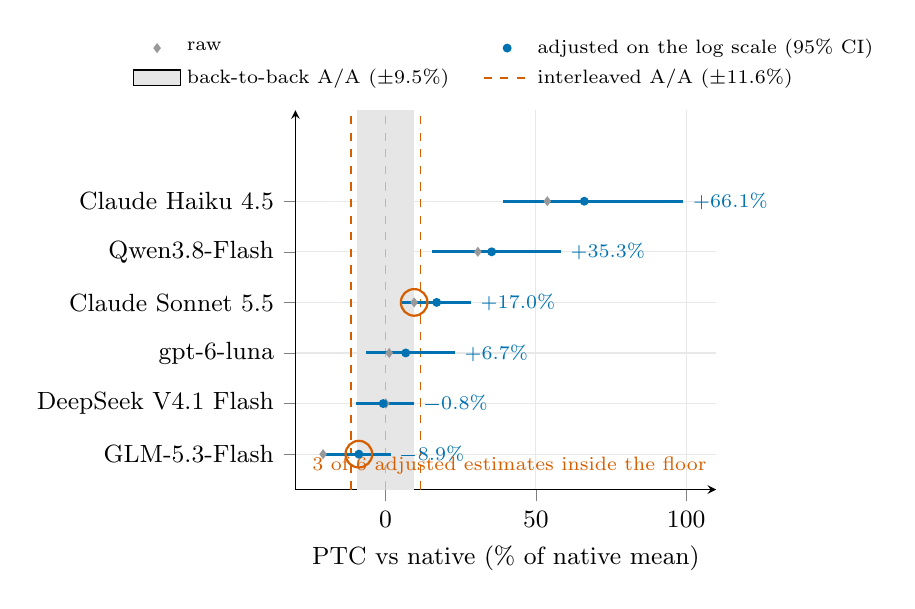
\begin{tikzpicture}
\definecolor{f4adj}{HTML}{0072B2}
\definecolor{f4raw}{HTML}{999999}
\definecolor{f4small}{HTML}{D55E00}
\begin{axis}[
  width=\linewidth-5.2cm, height=6.4cm, compat=1.18,
  xlabel={PTC vs native (\% of native mean)},
  xmin=-30, xmax=110,
  ytick={0,1,2,3,4,5},
  yticklabels={GLM-5.3-Flash,DeepSeek V4.1 Flash,gpt-6-luna,Claude Sonnet 5.5,Qwen3.8-Flash,Claude Haiku 4.5},
  ymin=-0.7, ymax=6.8,
  axis y line=left, axis x line=bottom, tick align=outside,
  grid=major, grid style={gray!18},
  yticklabel style={font=\small}, xticklabel style={font=\small}, xlabel style={font=\small}, ylabel style={font=\small},
  legend style={at={(0.5,1.03)}, anchor=south, legend columns=2, draw=none, font=\scriptsize, legend cell align=left, /tikz/every even column/.append style={column sep=10pt}},
  clip=false,
]
\addlegendimage{only marks, mark=diamond*, mark size=1.5pt, color=f4raw}
\addlegendentry{raw}
\addlegendimage{only marks, mark=*, mark size=1.4pt, color=f4adj}
\addlegendentry{adjusted on the log scale (95\% CI)}
\addlegendimage{area legend, fill=f4raw!25, draw=none}
\addlegendentry{back-to-back A/A ($\pm$9.5\%)}
\addlegendimage{f4small, dashed, line width=0.7pt}
\addlegendentry{interleaved A/A ($\pm$11.6\%)}
\fill[f4raw!25] (axis cs:-9.5,-0.7) rectangle (axis cs:9.5,6.8);
\draw[f4small, dashed, line width=0.7pt] (axis cs:-11.6,-0.7) -- (axis cs:-11.6,6.8);
\draw[f4small, dashed, line width=0.7pt] (axis cs:11.6,-0.7) -- (axis cs:11.6,6.8);
\draw[gray!55, dashed] (axis cs:0,-0.7) -- (axis cs:0,6.8);
\addplot[forget plot, only marks, mark=diamond*, mark size=1.5pt, color=f4raw] coordinates {(-20.8,0) (0.1,1) (1.2,2) (9.5,3) (30.7,4) (53.8,5)};
\addplot[forget plot, only marks, mark=*, mark size=1.4pt, color=f4adj] coordinates {(-8.9,0) (-0.8,1) (6.7,2) (17.0,3) (35.3,4) (66.1,5)};
\draw[f4adj, line width=1.1pt] (axis cs:-20.0,0) -- (axis cs:1.8,0);
\node[font=\scriptsize, anchor=west, text=f4adj] at (axis cs:1.8,0) {\textminus{}8.9\%};
\node[circle, draw=f4small, line width=0.8pt, inner sep=3.4pt] at (axis cs:-8.9,0) {};
\draw[f4adj, line width=1.1pt] (axis cs:-10.0,1) -- (axis cs:9.6,1);
\node[font=\scriptsize, anchor=west, text=f4adj] at (axis cs:9.6,1) {\textminus{}0.8\%};
\draw[f4adj, line width=1.1pt] (axis cs:-6.5,2) -- (axis cs:23.0,2);
\node[font=\scriptsize, anchor=west, text=f4adj] at (axis cs:23.0,2) {+6.7\%};
\draw[f4adj, line width=1.1pt] (axis cs:5.0,3) -- (axis cs:28.4,3);
\node[font=\scriptsize, anchor=west, text=f4adj] at (axis cs:28.4,3) {+17.0\%};
\node[circle, draw=f4small, line width=0.8pt, inner sep=3.4pt] at (axis cs:9.5,3) {};
\draw[f4adj, line width=1.1pt] (axis cs:15.6,4) -- (axis cs:58.3,4);
\node[font=\scriptsize, anchor=west, text=f4adj] at (axis cs:58.3,4) {+35.3\%};
\draw[f4adj, line width=1.1pt] (axis cs:39.1,5) -- (axis cs:99.1,5);
\node[font=\scriptsize, anchor=west, text=f4adj] at (axis cs:99.1,5) {+66.1\%};
\node[font=\scriptsize, anchor=south east, text=f4small] at (axis cs:110,-0.6) {3 of 6 adjusted estimates inside the floor};
\end{axis}
\end{tikzpicture}

\caption{The batch-1 effects adjusted on the log scale (percent of native mean, 95\% intervals;
$n = 31$ tasks per model) against the back-to-back A/A
half-width of 9.5\% (shaded) and the interleaved A/A half-width of 11.6\% (dashed); grey diamonds are
the raw estimates. Negative values mean PTC is cheaper than native. GLM's adjusted \mi{}8.9\% lies inside both, and Sonnet's raw +9.5\% on the edge of
the first and inside the second (ringed). Both floors are measured on DeepSeek only.}\label{fig:floor}\end{figure}

\paragraph{Resolution of the interval itself.} The study's first analyses used $B = 5{,}000$
bootstrap resamples. At that resolution Sonnet's lower bound sat at +0.28\%, a significant result, but
it fell below zero in 25 of 40 reseeds. At $B = 200{,}000$ it is \mi{}0.08\%. A classification that
depends on the random seed of the bootstrap is not a finding.

\paragraph{The replication.} After seeing the batch-1 results we filed a replication criterion on a
second suite before any of its data existed. \textbf{R1}: each of four providers keeps its batch-1 raw
classification (Qwen positive, GLM negative, luna null, DeepSeek null). \textbf{R2}: at least one
provider is positive and one negative. Replication requires R1 for all four plus R2. Neither holds
(Table~\ref{tab:r1}). R1 is 0 of 4 and stays 0 of 4 across 20 bootstrap seeds. R2 fails because no
provider is positive. Luna and DeepSeek moved from null to significantly negative, Qwen lost its
positive result, and GLM's interval crossed zero by 0.14 points. The quality check leaves every
tasks-b classification unchanged. On the log-adjusted scale the six-model spread fell from 75.1
points to 28.8; among the four pre-registered providers plotted in Figure~\ref{fig:replication} it is 24.0. Adjusting both suites for execution order does not
repair the failure: R1 becomes 1 of 4 and R2 still fails. No single divergence survives every analysis
convention, since on the additive scale all four pairs of intervals overlap. The pattern, however,
does not reproduce under any of them. Nor is the suite dependence an artefact of the shared order: in
the counterbalanced re-run (Table~\ref{tab:rerun}), as in the original, DeepSeek and luna are null on
batch 1 and significantly negative on tasks-b.

\begin{inlinetable}
\captionof{table}{Pre-registered replication criterion R1: filed batch-1 classification against the
tasks-b classification (raw contrast, 95\% interval).}\label{tab:r1}
\begin{tabular}{@{}llllr@{}}
\toprule
provider & batch 1 (filed) & tasks-b & tasks-b 95\% CI & R1 \\
\midrule
Qwen3.8-Flash & positive & null & [\mi{}3.93, +15.01] & differs \\
GLM-5.3-Flash & negative & null & [\mi{}21.12, +0.14] & differs \\
gpt-6-luna & null & negative & [\mi{}24.35, \mi{}8.55] & differs \\
DeepSeek V4.1 Flash & null & negative & [\mi{}37.46, \mi{}9.38] & differs \\
\bottomrule
\end{tabular}
\end{inlinetable}

\begin{figure}[htbp]\centering% Generated by tools/figures.mjs from analysis/position-adjust-6model-2026-10-09.json and analysis/position-adjust-batchb-2026-10-09.json - do not edit by hand.
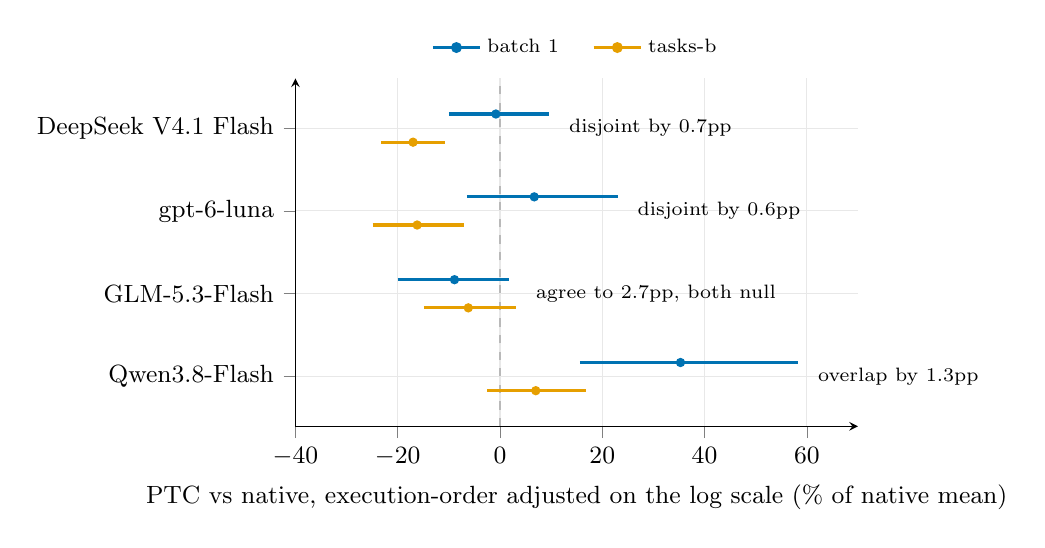
\begin{tikzpicture}
\definecolor{f2a}{HTML}{0072B2}
\definecolor{f2b}{HTML}{E69F00}
\begin{axis}[
  width=\linewidth-3.4cm, height=6.0cm, compat=1.18,
  xlabel={PTC vs native, execution-order adjusted on the log scale (\% of native mean)},
  xmin=-40, xmax=70,
  ytick={0,1,2,3},
  yticklabels={Qwen3.8-Flash,GLM-5.3-Flash,gpt-6-luna,DeepSeek V4.1 Flash},
  ymin=-0.6, ymax=3.60,
  axis y line=left, axis x line=bottom, tick align=outside,
  grid=major, grid style={gray!18},
  yticklabel style={font=\small}, xticklabel style={font=\small}, xlabel style={font=\small}, ylabel style={font=\small},
  legend style={at={(0.5,1.03)}, anchor=south, legend columns=2, draw=none, font=\scriptsize, /tikz/every even column/.append style={column sep=10pt}},
  clip=false,
]
\addlegendimage{f2a, line width=1.1pt, mark=*, mark size=1.4pt}
\addlegendentry{batch 1}
\addlegendimage{f2b, line width=1.1pt, mark=*, mark size=1.4pt}
\addlegendentry{tasks-b}
\draw[gray!55, dashed] (axis cs:0,-0.6) -- (axis cs:0,3.60);
\draw[f2a, line width=1.1pt] (axis cs:15.6,0.17) -- (axis cs:58.3,0.17);
\node[circle, fill=f2a, inner sep=1.2pt] at (axis cs:35.3,0.17) {};
\draw[f2b, line width=1.1pt] (axis cs:-2.5,-0.17) -- (axis cs:16.9,-0.17);
\node[circle, fill=f2b, inner sep=1.2pt] at (axis cs:7.0,-0.17) {};
\node[font=\scriptsize, anchor=west] at (axis cs:60.3,0) {overlap by 1.3pp};
\draw[f2a, line width=1.1pt] (axis cs:-20.0,1.17) -- (axis cs:1.8,1.17);
\node[circle, fill=f2a, inner sep=1.2pt] at (axis cs:-8.9,1.17) {};
\draw[f2b, line width=1.1pt] (axis cs:-14.9,0.83) -- (axis cs:3.1,0.83);
\node[circle, fill=f2b, inner sep=1.2pt] at (axis cs:-6.2,0.83) {};
\node[font=\scriptsize, anchor=west] at (axis cs:5.1,1) {agree to 2.7pp, both null};
\draw[f2a, line width=1.1pt] (axis cs:-6.5,2.17) -- (axis cs:23.0,2.17);
\node[circle, fill=f2a, inner sep=1.2pt] at (axis cs:6.7,2.17) {};
\draw[f2b, line width=1.1pt] (axis cs:-24.9,1.83) -- (axis cs:-7.1,1.83);
\node[circle, fill=f2b, inner sep=1.2pt] at (axis cs:-16.2,1.83) {};
\node[font=\scriptsize, anchor=west] at (axis cs:25.0,2) {disjoint by 0.6pp};
\draw[f2a, line width=1.1pt] (axis cs:-10.0,3.17) -- (axis cs:9.6,3.17);
\node[circle, fill=f2a, inner sep=1.2pt] at (axis cs:-0.8,3.17) {};
\draw[f2b, line width=1.1pt] (axis cs:-23.2,2.83) -- (axis cs:-10.8,2.83);
\node[circle, fill=f2b, inner sep=1.2pt] at (axis cs:-17.0,2.83) {};
\node[font=\scriptsize, anchor=west] at (axis cs:11.6,3) {disjoint by 0.7pp};
\end{axis}
\end{tikzpicture}

\caption{The replication: tasks-b against batch 1 for the four pre-registered providers, both adjusted
for execution order on the log scale, with 95\% intervals (batch 1: $n = 31$ tasks; tasks-b: $n = 40$).
Negative values mean PTC is cheaper than native. On tasks-b the four providers span 24.0 points
(Qwen $+6.96$ to DeepSeek $\mi{}17.04$).}\label{fig:replication}\end{figure}

Both Anthropic models, collected on tasks-b as an extension, also move from positive to null (Haiku
+6.2\% over 18 tasks, Sonnet \mi{}0.5\% over 40). Three of the six pitfalls feed into this failure:
the first reading's significant GLM result was partly an execution-order effect (Pitfall~4), Haiku's
penalty is entangled with its failures (Pitfall~5), and most effects sit near the noise floor.
Without the second suite, the first reading would have stood.

\section{What survives: code mode after the corrections}\label{sec:survives}

With the six pitfalls addressed as far as the data allow, the following can be said about code mode.

\paragraph{The cost effect depends on the model and the suite.} After adjusting for execution order,
code mode's effect on batch 1 ranges from \mi{}8.9\% to +66.1\% (Appendix Figure~\ref{fig:penalty}), and the
pattern did not replicate. The counterbalanced re-run agrees: on batch 1 no model is significantly
cheaper under code mode, while on tasks-b DeepSeek (\mi{}16.8\%) and luna (\mi{}19.0\%) are, as in the
original collection. Those two savings are the only ones the study reproduces, and only on one suite.
The one robust case is Claude Haiku 4.5 on batch 1, on which code mode is dearer per solved task
and less reliable, in both collections (+78.4\% per task and 48 against 62 solved in
the re-run). On tasks-b the per-solved direction is the same (+62.4\%) but the per-task and both-solved
intervals include zero.

\paragraph{The price ratio does not explain it.} The study was motivated by the idea that code mode
shifts cost toward output, so its penalty should grow with the output:input price ratio. The
pre-registered primary test (H1) is inconclusive: the slope of the penalty on output share is
$b_1 = +0.00467$ [\mi{}0.00566, +0.01579], and on tasks-b it is negative. The pre-registered secondary,
a gap of more than 5 points between the mean penalty at ratio 5.00 and at 3.33, is nominally met
(42.3 points). But ratio 3.33 is one model, and the three models sharing ratio 5.00 differ among
themselves by 59.5 of the 75.1-point adjusted spread (79.2\%; Appendix Figure~\ref{fig:penalty}). The ratio is read off the provider
cells, not manipulated, and is confounded with model and cache regime. These data neither establish
nor exclude a ratio effect.

\paragraph{Code mode reduces requests, but that is not a cost saving.} Native mode made more model
requests per run than PTC on both suites, +2.228 [+1.228, +3.360] on batch 1 and +8.378 [+7.244,
+9.606] on tasks-b, as pre-registered (H3). The batch-1 effect rests largely on gpt-6-luna (20.4
against 12.1 requests per run). Without it the interval includes zero, and Qwen and Haiku show no
difference. Because native and PTC differ in whether calls can be batched as well as in tool count, we
read H3 as ``PTC reduces request count'', not as an effect of schema count. Request savings did not
predict cost savings: the two models with the largest savings on batch 1 have null cost effects.

\paragraph{Caching explains at most one model.} Prefix retention, the share of a cached prefix the
provider still serves from cache, falls under PTC only on Qwen (\mi{}0.065 [\mi{}0.078, \mi{}0.052]),
and there it is confounded with breakpoint placement (Pitfall~2). On Haiku the retention loss is
\mi{}0.005, far too small to explain its penalty. Elsewhere retention is flat at 0.99--1.00.

\paragraph{Harness rankings are only weakly shared across models.} Over the eight non-terse arms, the
median Spearman correlation between two models' cost rankings is 0.238 on batch 1. That is more than
independent random rankings would give ($p = 0.047$), but on tasks-b the median is 0.024. Within a
model, 74\% of adjacent pairs in the cost ranking are statistically indistinguishable on batch 1 and
61\% on tasks-b (54 pairs across all six models, including Anthropic external arms priced at the
miss-rate default of Pitfall~\ref{sec:p3}). Pairs of DSH arms tie in 18 of 24 on both suites, pairs of two external harnesses in
half (Figure~\ref{fig:ties}). Adjusting for execution order changes these figures by at most two
points. A ranking measured with one model is a weak guide to another, and most steps between harnesses
are not resolved at this sample size.

\begin{figure}[htbp]\centering% Generated by tools/figures.mjs from analysis/ranking-adjusted-2026-10-10.json - do not edit by hand.
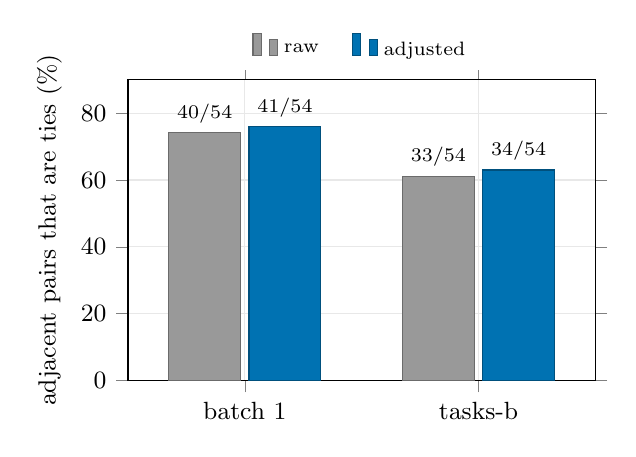
\begin{tikzpicture}
\definecolor{f3raw}{HTML}{999999}
\definecolor{f3adj}{HTML}{0072B2}
\begin{axis}[
  width=0.62\linewidth, height=5.4cm, compat=1.18, ybar=3pt, bar width=26pt,
  ylabel={adjacent pairs that are ties (\%)},
  yticklabel style={font=\small}, xticklabel style={font=\small}, xlabel style={font=\small}, ylabel style={font=\small},
  symbolic x coords={batch 1,tasks-b}, xtick=data,
  ymin=0, ymax=90,
  enlarge x limits=0.5,
  nodes near coords, point meta=explicit symbolic, every node near coord/.append style={font=\scriptsize},
  legend style={at={(0.5,1.03)}, anchor=south, legend columns=2, draw=none, font=\scriptsize, /tikz/every even column/.append style={column sep=10pt}},
  tick align=outside, grid=major, grid style={gray!18},
]
\addplot[fill=f3raw, draw=f3raw!70!black] coordinates {(batch 1,74.1) [40/54] (tasks-b,61.1) [33/54]};
\addlegendentry{raw}
\addplot[fill=f3adj, draw=f3adj!70!black] coordinates {(batch 1,75.9) [41/54] (tasks-b,63.0) [34/54]};
\addlegendentry{adjusted}
\end{axis}
\end{tikzpicture}

\caption{Adjacent arm pairs in each model's cost ranking that are statistically indistinguishable, raw
and adjusted for execution order (ties out of 54 adjacent pairs). The 54 pairs include Anthropic
external arms priced at the miss-rate default used when the cache split is missing.}\label{fig:ties}\end{figure}

\section{A checklist for measuring agent cost}\label{sec:checklist}

Table~\ref{tab:checklist} collects one practice per pitfall. None is expensive if planned before
collection. Several are expensive to repair afterwards, which is the situation this study was in.

\begin{inlinetable}
\captionof{table}{Practices for measuring the cost of agents, one per pitfall.}\label{tab:checklist}
\begin{tabular}{@{}lL{5.0cm}L{7.6cm}@{}}
\toprule
 & pitfall & practice \\
\midrule
1 & Token volume is not cost & Price from the provider's own usage block, including the cache split; report billed and cold-cache cost side by side. \\
2 & Cache configuration is part of the treatment & Report each condition's cache regime (automatic, declared, where the breakpoints sit); check that no arm falls under a provider's minimum cacheable length; never inject declarations into a client that declares its own. \\
3 & Accounting can be missing; meters fail silently & Reconcile computed cost against the provider's ledger; make cost tools fail on unknown models or missing cache splits instead of defaulting; report brackets where accounting is missing. \\
4 & Execution order carries cost & Randomise the run order independently per configuration and matrix; counterbalance which arm leads in a paired contrast; record the slot; check for order effects before analysing. \\
5 & Cost without quality misleads & Test whether arms solve the same tasks; report cost per solved task and the contrast on commonly solved tasks; grade against suites the agent cannot edit. \\
6 & One suite, one sample, one resolution & Run an interleaved A/A to measure the noise floor and size the task set from it; use enough bootstrap resamples to make classifications seed-stable; replicate on a second suite before claiming a direction. \\
\bottomrule
\end{tabular}
\end{inlinetable}


\section{Use of AI tools}\label{sec:aiuse}
The authors used large language model (LLM) assistants extensively in this work. They helped
design and set up the experiments and guided their execution; they also helped build the
surrounding infrastructure, including tooling and the measurement harness. The first author wrote
an initial rough draft of the manuscript, which LLM assistants substantially rewrote and expanded
into the present text. The authors directed the project and chose the research questions;
Alexander Feurer contributed substantially to the initial research idea; Max Reischl ran and
oversaw the experiments. Both authors reviewed the final manuscript and take full responsibility
for all content, numbers and citations. LLM assistants are not authors of this paper.

\section{Limitations}\label{sec:limitations}

\paragraph{One harness carries the code-mode contrast.} Code mode was tested inside DSH only, so the
code-mode findings concern DSH's implementation, and we wrote its study conditions. The pitfalls do not
depend on this, but the code-mode results would be stronger with a second harness that offers a code
mode.

\paragraph{Model, provider and cache regime are confounded.} Each model comes from one provider with
one cache regime and wire protocol. Only within Anthropic can model be separated from provider, and
there the adjusted effect still differs by 49 points.

\paragraph{The study carries its own pitfalls.} The shared execution order affects both suites, and the
adjustment for it rests on an assumption the design cannot test. The counterbalanced re-run removes
this for the central contrast on five models, but not for Sonnet, the eight other arms or the
harness rankings, which still rest on the adjustment. The re-run is a later collection, so it also
carries drift (native cost per cell moved by up to 8\%). The sample
is below what the measured noise floor calls for, and both floors are measured on one model. Haiku's tasks-b row covers 353 analysed cells from 18 of 40 tasks that are not a random subset. The
pre-registration was amended 23 times, so its freeze is nominal (Appendix~\ref{app:prereg}). Several
figures circulated during the study were later withdrawn (Appendix~\ref{app:corrections}). The pilots
behind Pitfall~2 and the incidents in Pitfall~3 come from the development record and are not part of
the checksummed artifact.

\paragraph{Lost data.} An earlier, larger panel, including a seventh model, was destroyed on 2026-10-02
together with its logs. Nothing here depends on it.

\section{Conclusion}\label{sec:conclusion}

A careful study of whether code mode makes coding agents cheaper---protocol fixed in advance with 23
documented amendments (Appendix~\ref{app:prereg})---reached a mixed
answer. No model was significantly cheaper on batch 1; on the second suite DeepSeek and gpt-6-luna were, and a counterbalanced re-run reproduced both savings. The batch-1 pattern did not replicate. Reaching
even that answer required avoiding six pitfalls, and at each of them a standard measurement practice
would have changed the conclusion or mis-sized it. Priced without cache accounting, code mode looks cheaper on 4 of 6
models (Table~\ref{tab:coldbilled}); the point-estimate sign flips on half, and those three billed intervals include zero (only Haiku survives Holm on batch 1). Under one cache declaration it is never cached. Without an outside ledger, the cost tool
reports more than was spent. With a shared run order, a significant saving appears that neither the
adjustment nor a counterbalanced re-run supports (the order effect itself is significant in 1 of 9 re-run rows; GLM's reversal sits within native-arm drift).
Without a quality check, a doubling of cost per solved task looks like +54\%. Without a second suite,
the first suite's pattern would have stood. Cost is now routinely reported for agents. It should be
measured with the same care as accuracy.

\bibliographystyle{tmlr}
\bibliography{refs}

\clearpage
\begin{appendices}

\section{Pre-registration status}\label{app:prereg}

\begin{inlinetable}
\captionof{table}{Confirmatory hypotheses on batch 1 (six models) and their verdicts under the filed
decision rules.}\label{tab:hypotheses}
\begin{tabular}{@{}L{5.0cm}L{7.2cm}L{3.4cm}@{}}
\toprule
hypothesis & result & verdict \\
\midrule
H1 (primary): the PTC penalty rises with output share & $b_1 = +0.00467$ [\mi{}0.00566, +0.01579], $n = 186$ & inconclusive \\
H2: terseness reduces the PTC penalty & mean $d = +0.00151$ [\mi{}0.00010, +0.00354], Wilcoxon $p = 0.80$ & inconclusive \\
H3: 24 schemas rather than 1 increase requests & +2.228 [+1.228, +3.360] & supported \\
H4: cache hit rate does not predict arm cost & $b_C = +0.11157$ [+0.06235, +0.17140] & refuted \\
\bottomrule
\end{tabular}
\end{inlinetable}

\begin{itemize}
\item H5 (exploratory, no formal test) predicted that harness cost rankings are not stable across
providers; \S\ref{sec:survives} reports the statistics.
\item The filing was amended 23 times. Versions 1--3 each named a freeze commit that did not contain
them, and version 4 edited the text after its tag. Amendments 21--23 post-date the last tag.
\item H1 was refuted on the four cheaper providers and became inconclusive when the Anthropic models
were added. A mixed model with a task random intercept gives the same $b_1$. On the four
pre-registered providers on tasks-b, $b_1 = \mi{}0.0125$ [\mi{}0.0203, \mi{}0.0050].
\item The Holm family was filed with 12 members (4 cost, 8 solve-rate) and grew to 18 when the
Anthropic models were added, after their collection. Of the 18, two survive, both Haiku's: the PTC
cost contrast ($p = 0.00005$) and the PTC-to-PTC-terse solve-rate contrast ($p = 0.00014$). Qwen's
cost contrast ($p = 0.0056$) fails only through the correction. On tasks-b the filed family of 12
has two survivors, DeepSeek ($p = 0.0001$) and luna ($p = 0.0003$), both saying PTC is cheaper.
\item The filing exempts only H1 and H2 from correction by name. H3 is reported uncorrected, and its
$p$ of about $3\times10^{-5}$ survives any family we could construct.
\item The test-editing rule (report as measured, exclude nothing, publish two sensitivities) was
committed before its effect was computed. The replication criterion and the Anthropic extension
verdict were filed before any tasks-b record existed.
\item The counterbalanced re-run (\S\ref{sec:p4}, Appendix~\ref{app:rerun}) was filed after the
original results were known but before any re-run record existed, and was not amended. Of its two
predictions, the order-bias prediction holds at the threshold (5 of 8) and the A/A prediction fails
in its first part (\S\ref{sec:p6}).
\end{itemize}

\section{Robustness}\label{app:robust}

\paragraph{Scale of the execution-order adjustment.} By held-out prediction, the log scale wins 9 of 12
model$\times$suite comparisons, by up to 1.8$\times$. Four of those wins, and all three additive wins,
are marginal. The scales disagree about a classification in two rows: GLM (null on both adjusted
scales) and Sonnet (positive on log, null on additive).

\paragraph{Arm string.} With \texttt{dsh:ptc-opt} against \texttt{dsh:native-opt} as the central
pair, every tasks-b sign is kept (DeepSeek \mi{}19.4\%, GLM \mi{}7.0\%, Qwen +3.9\%, Haiku +10.2\%,
Sonnet +1.4\%, luna \mi{}8.8\%), but luna moves from negative to null. On batch 1 the pairs differ in
size and sometimes in sign (Haiku +53.8\% against +79.0\%, GLM \mi{}20.8\% against \mi{}12.7\%,
DeepSeek +0.1\% against \mi{}10.1\%). Under the variant pair no provider's batch-1 and tasks-b
intervals separate.

\paragraph{Seeds.} On batch 1, Qwen is positive on seed 1 (+37.4\% [+18.7, +57.3]) and null on seed 2
(+24.0\% [\mi{}3.5, +58.3]). Haiku is positive on both, and Sonnet only on seed 2. On tasks-b, GLM is
negative on seed 1 and null on seed 2.

\paragraph{Leave one model out.} The adjacent-step tie fraction stays within 71.1--80.0\% (batch 1)
and 57.8--64.4\% (tasks-b). The median $\rho$ ranges over 0.119--0.262 and \mi{}0.190 to +0.071. H3 on
batch 1 ranges from 2.206 to 2.703 for five of the six drops, and is +1.010 [\mi{}0.081, +2.223]
without luna. On tasks-b it ranges from 6.379 to 9.642.

\begin{figure}[htbp]\centering% Generated by tools/figures.mjs from analysis/position-adjust-6model-2026-10-09.json - do not edit by hand.
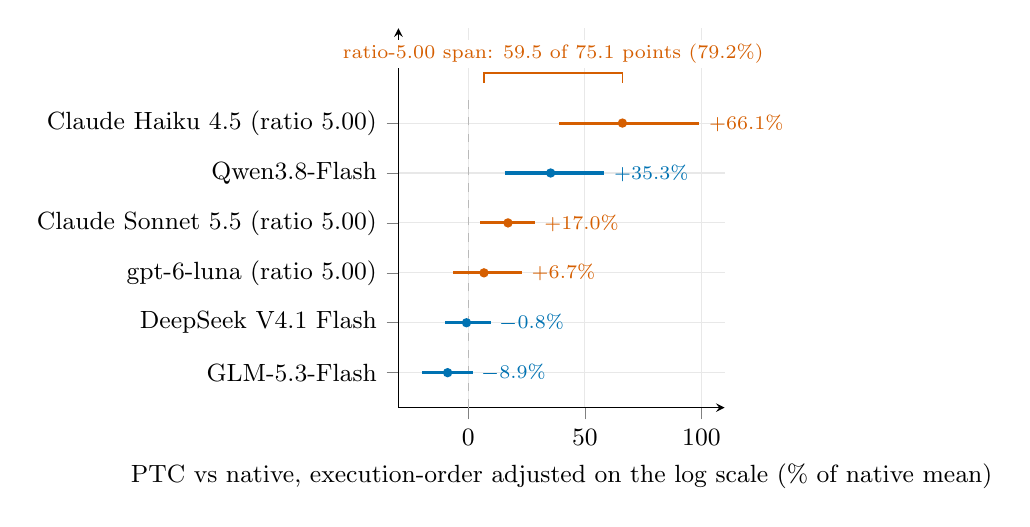
\begin{tikzpicture}
\definecolor{f1main}{HTML}{0072B2}
\definecolor{f1r5}{HTML}{D55E00}
\begin{axis}[
  width=\linewidth-6.4cm, height=6.4cm, compat=1.18,
  xlabel={PTC vs native, execution-order adjusted on the log scale (\% of native mean)},
  xmin=-30, xmax=110,
  ytick={0,1,2,3,4,5},
  yticklabels={GLM-5.3-Flash,DeepSeek V4.1 Flash,gpt-6-luna (ratio 5.00),Claude Sonnet 5.5 (ratio 5.00),Qwen3.8-Flash,Claude Haiku 4.5 (ratio 5.00)},
  yticklabel style={font=\small}, xticklabel style={font=\small}, xlabel style={font=\small}, ylabel style={font=\small},
  ymin=-0.7, ymax=6.9,
  axis y line=left, axis x line=bottom, tick align=outside,
  grid=major, grid style={gray!18},
  clip=false,
]
\draw[gray!55, dashed] (axis cs:0,-0.7) -- (axis cs:0,5.6);
\draw[f1r5, line width=0.6pt] (axis cs:6.7,5.8) -- (axis cs:6.7,6.0) -- (axis cs:66.1,6.0) -- (axis cs:66.1,5.8);
\node[font=\scriptsize, anchor=south, text=f1r5, fill=white, inner sep=1.5pt] at (axis cs:36.4,6.1) {ratio-5.00 span: 59.5 of 75.1 points (79.2\%)};
\draw[f1main, line width=1.1pt] (axis cs:-20.0,0) -- (axis cs:1.8,0);
\node[circle, fill=f1main, inner sep=1.2pt] at (axis cs:-8.9,0) {};
\node[font=\scriptsize, anchor=west, text=f1main] at (axis cs:1.8,0) {\textminus{}8.9\%};
\draw[f1main, line width=1.1pt] (axis cs:-10.0,1) -- (axis cs:9.6,1);
\node[circle, fill=f1main, inner sep=1.2pt] at (axis cs:-0.8,1) {};
\node[font=\scriptsize, anchor=west, text=f1main] at (axis cs:9.6,1) {\textminus{}0.8\%};
\draw[f1r5, line width=1.1pt] (axis cs:-6.5,2) -- (axis cs:23.0,2);
\node[circle, fill=f1r5, inner sep=1.2pt] at (axis cs:6.7,2) {};
\node[font=\scriptsize, anchor=west, text=f1r5] at (axis cs:23.0,2) {+6.7\%};
\draw[f1r5, line width=1.1pt] (axis cs:5.0,3) -- (axis cs:28.4,3);
\node[circle, fill=f1r5, inner sep=1.2pt] at (axis cs:17.0,3) {};
\node[font=\scriptsize, anchor=west, text=f1r5] at (axis cs:28.4,3) {+17.0\%};
\draw[f1main, line width=1.1pt] (axis cs:15.6,4) -- (axis cs:58.3,4);
\node[circle, fill=f1main, inner sep=1.2pt] at (axis cs:35.3,4) {};
\node[font=\scriptsize, anchor=west, text=f1main] at (axis cs:58.3,4) {+35.3\%};
\draw[f1r5, line width=1.1pt] (axis cs:39.1,5) -- (axis cs:99.1,5);
\node[circle, fill=f1r5, inner sep=1.2pt] at (axis cs:66.1,5) {};
\node[font=\scriptsize, anchor=west, text=f1r5] at (axis cs:99.1,5) {+66.1\%};
\end{axis}
\end{tikzpicture}

\caption{PTC against native on batch 1, adjusted for execution order on the log scale (percent of
native mean, 95\% intervals; $n = 31$ tasks). Negative values mean PTC is cheaper than native. The three models with an output:input price ratio of 5.00 (red) span
59.5 of the 75.1-point range (79.2\%).}\label{fig:penalty}\end{figure}

\paragraph{Replication under the adjustment.} On the log-adjusted scale luna moved from +6.7\% to
\mi{}16.2\% and DeepSeek from \mi{}0.8\% to \mi{}17.0\%, with intervals disjoint by 0.6 and 0.7 points.
Qwen fell from +35.3\% to +7.0\%, and GLM moved from \mi{}8.9\% to \mi{}6.2\%, null on both suites.

\section{The Anthropic extension on tasks-b}\label{app:extension}

\begin{inlinetable}
\captionof{table}{Anthropic extension on tasks-b, per cell and per solved task. Haiku's cells are those
that ran before the account limit (353 analysed cells from 18 of 40 tasks).}\label{tab:extension}
\begin{tabular}{@{}lrrrr@{}}
\toprule
arm & cells & solved & per cell & per solved task \\
\midrule
Haiku \texttt{dsh:native} & 36 & 26 (72.2\%) & \$0.2851 & \$0.3948 \\
Haiku \texttt{dsh:ptc} & 36 & 17 (47.2\%) & \$0.3028 & \$0.6412 \\
Sonnet \texttt{dsh:native} & 80 & 78 (97.5\%) & \$0.1363 & \$0.1398 \\
Sonnet \texttt{dsh:ptc} & 80 & 77 (96.3\%) & \$0.1356 & \$0.1409 \\
\bottomrule
\end{tabular}
\end{inlinetable}

The tasks-b plan required this per-solved-task reading for the Haiku row before the full matrix ran.
Over the full 40-task design, counting cells lost to the outage as unsolved, 10 pairs are solved by
native only and 1 by PTC only (exact McNemar $p = 0.0117$). Haiku's tasks-b interval is
[\mi{}7.35, +19.67] and Sonnet's [\mi{}7.92, +5.98].

\section{The counterbalanced re-run}\label{app:rerun}

The re-run used the same harness version, tasks, grading, seeds and gateway as the original, with
DSH only, so that no external harness was spent on. Its matrices: batch 1 (31 tasks, 2 seeds, 124
cells) on DeepSeek, GLM, Qwen, luna and Haiku; tasks-b (40 tasks, 2 seeds, 160 cells) on the four
cheaper models; and the interleaved A/A on DeepSeek (124 cells). Every matrix was collected in full.
The re-run cost \$46.48 at the gateway meter against a filed stop of \$70. For Haiku, the only
matrix on its provider account in that window, the account balance fell by \$20.61 (\$57.90 to
\$37.29, read from the provider console) against \$20.60 at the meter: on the DSH arms, whose
requests carry the cache split, meter and bill agree, unlike the external harnesses of
\S\ref{sec:p3}.

\begin{inlinetable}
\captionof{table}{Quality in the re-run: cells solved by native/PTC (of 62 per arm on batch 1 and 80
on tasks-b), discordant pairs (native only : PTC only) with the exact McNemar test, and the contrast on
cells both modes solved (95\% task-clustered bootstrap, $B = 200{,}000$).}\label{tab:rerunquality}
\setlength{\tabcolsep}{4pt}
\begin{tabular}{@{}llrrrrl@{}}
\toprule
suite & model & solved & discordant & McNemar $p$ & cells & both-solved contrast \\
\midrule
batch 1 & DeepSeek V4.1 Flash & 62/62 & 0 : 0 & 1.00 & 62 & +0.93\% [\mi{}9.96, +12.67] \\
 & GLM-5.3-Flash & 62/62 & 0 : 0 & 1.00 & 62 & +15.38\% [+0.97, +32.95] \\
 & Qwen3.8-Flash & 62/60 & 2 : 0 & 0.50 & 60 & +36.32\% [+24.57, +49.00] \\
 & gpt-6-luna & 61/61 & 1 : 1 & 1.00 & 60 & \mi{}1.31\% [\mi{}11.29, +8.81] \\
 & Claude Haiku 4.5 & 62/48 & 14 : 0 & 0.00012 & 48 & +107.05\% [+72.67, +146.15] \\
\midrule
tasks-b & DeepSeek V4.1 Flash & 78/78 & 2 : 2 & 1.00 & 76 & \mi{}19.08\% [\mi{}34.61, \mi{}6.65] \\
 & GLM-5.3-Flash & 78/71 & 8 : 1 & 0.039 & 70 & \mi{}2.29\% [\mi{}17.25, +14.80] \\
 & Qwen3.8-Flash & 74/74 & 3 : 3 & 1.00 & 71 & +11.52\% [+1.01, +22.70] \\
 & gpt-6-luna & 76/75 & 5 : 4 & 1.00 & 71 & \mi{}23.59\% [\mi{}32.82, \mi{}14.93] \\
\bottomrule
\end{tabular}
\end{inlinetable}

Three tooling defects surfaced during collection, each stopped by the pipeline before it could
affect a record, and each fixed and recorded in the filed plan. The first A/A smoke failed at its pilot
because a process the harness spawned still held the shared A/A workdir when the twin started, so
its clean is now retried until the handle is released. The pilot stage then judged records left in a
shared scratch file by an earlier attempt, so each pilot is now judged on its own records only. And
the collector priced Haiku at an all-harness Anthropic average, which put the matrix above its filed
ceiling before it started, so the plan now carries Haiku's filed DSH cost. Separately, the Qwen
tasks-b collection stopped at 124 of 160 cells when its processes were lost, and it was resumed
under the same matrix identifier, so the counterbalanced assignment held. One cell that the
interruption left with a malformed record was run again under the plan's retry rule. Its two records
are averaged, as for every repeated cell.

\section{Corrections to earlier figures}\label{app:corrections}

Figures from earlier drafts of this study that are withdrawn or corrected:
\begin{itemize}
\item An execution-order ``standardisation'' that roughly halved every effect (Haiku +25.41\%) used an
estimator that summarised both arms' records as one arm's. It is withdrawn. Both legitimate corrections,
a slot fixed-effect regression (+52.97\%) and the paired estimator used here (+51.79\% additive), leave
Haiku near its raw value.
\item An earlier A/A pair compared two differently named arms whose first requests differed by 20--30
bytes. Its floors (46.2\%, then 7.7\%) are withdrawn in favour of the repeated-baseline design of
\S\ref{sec:p6}.
\item External-harness prefix retention on Anthropic (0.560, 0.451) mixed four unmeasured external arms,
coded as 0, with four DSH arms. No external-harness retention on the OpenAI-compatible path exists.
\item Anthropic per-run costs of \$0.105--0.233 (Haiku) and \$0.082--0.202 (Sonnet) were unreconciled
per-model bounds. Table~\ref{tab:cost} gives the ledger-reconciled brackets.
\item Sonnet's batch-1 contrast was reported as significant at $B = 5{,}000$. It is null at
$B = 200{,}000$.
\item An earlier draft headlined a sign disagreement between providers and a penalty independent of
the price ratio. The sign disagreement did not replicate and does not survive the execution-order
adjustment, and the ratio question is open (\S\ref{sec:survives}).
\end{itemize}

\section{Artifact and reproducibility}\label{app:artifact}

Every number in the main matrices, the replication suite, the A/A run and the OpenCode pilot is
re-derived from archived run records and gateway logs by commands recorded in
\texttt{artifact/MANIFEST.json}, which checksums 126 files across two scopes: the batch-1 matrices as
signed off on 2026-10-04, and the later material (the tasks-b suite, the execution-order adjustment,
the ablations, the mixed-effects fit, the ranking and retention sensitivities, the test-edit
incidence, the verdict seed stability, the A/A run, the retention pilot, the Anthropic cost bracket,
the common-slot check, the quality check, the batch-1 contrasts at $B = 200{,}000$, and the
counterbalanced re-run with its interleaved A/A).
\texttt{node tools/artifact.mjs \mbox{-{}-verify}} fails on any drift. The per-model Anthropic brackets
are arithmetic on the filed bracket and the ledger (\S\ref{sec:p3}). The Anthropic cache A/B
(Table~\ref{tab:anthropicab}), the billing reconciliation of \S\ref{sec:measurement} and the
pipeline incidents of \S\ref{sec:p3} come from the development pilots, whose records ship as
documents but whose raw logs are not in the manifest.

\begin{inlinetable}
\captionof{table}{Where each result is filed (all under \texttt{analysis/}).}\label{tab:files}
\begin{tabular}{@{}L{5.6cm}L{10.4cm}@{}}
\toprule
result & output (tool) \\
\midrule
Tables~\ref{tab:raw}, \ref{tab:r1}; family tests & \texttt{panel-analysis-6model-2026-10-09.json}, \texttt{panel-analysis-batchb-four-2026-10-09.json} (\texttt{panel-analysis.mjs}) \\
Table~\ref{tab:adjusted}; Figures~\ref{fig:penalty}, \ref{fig:replication} & \texttt{position-adjust-6model-2026-10-09.json}, \texttt{position-adjust-batchb-2026-10-09.json} (\texttt{position-adjust.mjs}) \\
Table~\ref{tab:quality} & \texttt{quality-guard-2026-10-10.json} (\texttt{quality-guard.mjs}) \\
Table~\ref{tab:coldbilled}, retention & \texttt{prefix-retention.json}, \texttt{prefix-retention-ci-2026-10-10.json} \\
Replication verdict, seed stability & \texttt{replication-verdict-batchb-2026-10-09.json}, \texttt{verdict-seed-stability-2026-10-10.json} \\
H1--H4, Table~\ref{tab:hypotheses} & \texttt{hypotheses-6model-2026-10-09.json}, \texttt{mixed-effects-6model-2026-10-04.json} \\
Rankings, Figure~\ref{fig:ties} & \texttt{ranking-adjusted-2026-10-10.json}, \texttt{ablations-2026-10-09.json} \\
Table~\ref{tab:cost}, OpenCode pilot & \texttt{anthropic-cost-bracket-2026-10-10.json}, \texttt{retention-pilot-2026-10-10.json} \\
A/A, Figure~\ref{fig:floor} & \texttt{aa-placebo-2026-10-10.json} (\texttt{aa-analysis.mjs}) \\
Test editing & \texttt{test-edit-sensitivity-6model-2026-10-04.json}, \texttt{test-edit-incidence-2026-10-10.json} \\
Common-slot check & \texttt{common-f-infeasibility-2026-10-10.json} \\
Tables~\ref{tab:rerun}, \ref{tab:rerunquality}; interleaved A/A & \texttt{rerun-compare-2026-10-11.json} (\texttt{rerun-compare.mjs}) \\
\bottomrule
\end{tabular}
\end{inlinetable}

The figures are generated from these files by \texttt{node tools/figures.mjs}. The methods record,
the pre-registration with its amendments, the replication plan and the defect records ship with the
artifact. The long-form research record of the study, with every intermediate and withdrawn result, is
\texttt{PAPER.md}.

\paragraph{Code and data availability.}
The gateway, run records, logs, analysis code and checksummed artifact are at
\url{https://github.com/Max6617/betterharness}, commit \texttt{71a6627}
(\texttt{71a662728c768782e55c91a1e94775f75f8a9956}), under the MIT License
(Copyright (c)~2026 Max Reischl and Alexander Feurer).
[Zenodo DOI to be added on release].

\end{appendices}

\end{document}
